%%%%%%%%%%%%%%%%%%%%%%%%%%%%%%%%%%%%%%%%%
% The Legrand Orange Book
% LaTeX Template
% Version 2.2 (30/3/17)
%
% This template has been downloaded from:
% http://www.LaTeXTemplates.com
%
% Original author:
% Mathias Legrand (legrand.mathias@gmail.com) with modifications by:
% Vel (vel@latextemplates.com)
%
% License:
% CC BY-NC-SA 3.0 (http://creativecommons.org/licenses/by-nc-sa/3.0/)
%
% Compiling this template:
% This template uses biber for its bibliography and makeindex for its index.
% When you first open the template, compile it from the command line with the 
% commands below to make sure your LaTeX distribution is configured correctly:
%
% 1) pdflatex main
% 2) makeindex main.idx -s StyleInd.ist
% 3) biber main
% 4) pdflatex main x 2
%
% After this, when you wish to update the bibliography/index use the appropriate
% command above and make sure to compile with pdflatex several times 
% afterwards to propagate your changes to the document.
%
% This template also uses a number of packages which may need to be
% updated to the newest versions for the template to compile. It is strongly
% recommended you update your LaTeX distribution if you have any
% compilation errors.
%
% Important note:
% Chapter heading images should have a 2:1 width:height ratio,
% e.g. 920px width and 460px height.
%
%%%%%%%%%%%%%%%%%%%%%%%%%%%%%%%%%%%%%%%%%

%----------------------------------------------------------------------------------------
%	PACKAGES AND OTHER DOCUMENT CONFIGURATIONS
%----------------------------------------------------------------------------------------

\documentclass[11pt,fleqn]{book} % Default font size and left-justified equations



%----------------------------------------------------------------------------------------

%%%%%%%%%%%%%%%%%%%%%%%%%%%%%%%%%%%%%%%%%
% The Legrand Orange Book
% Structural Definitions File
% Version 2.0 (9/2/15)
%
% Original author:
% Mathias Legrand (legrand.mathias@gmail.com) with modifications by:
% Vel (vel@latextemplates.com)
% 
% This file has been downloaded from:
% http://www.LaTeXTemplates.com
%
% License:
% CC BY-NC-SA 3.0 (http://creativecommons.org/licenses/by-nc-sa/3.0/)
%
%%%%%%%%%%%%%%%%%%%%%%%%%%%%%%%%%%%%%%%%%

%----------------------------------------------------------------------------------------
%	VARIOUS REQUIRED PACKAGES AND CONFIGURATIONS
%----------------------------------------------------------------------------------------

\usepackage[top=3cm,bottom=3cm,left=3cm,right=3cm,headsep=10pt,a4paper]{geometry} % Page margins

\usepackage{graphicx} % Required for including pictures
\graphicspath{{Pictures/}} % Specifies the directory where pictures are stored

\usepackage{lipsum} % Inserts dummy text

\usepackage{tikz} % Required for drawing custom shapes

\usepackage[english]{babel} % English language/hyphenation

\usepackage{enumitem} % Customize lists
\setlist{nolistsep} % Reduce spacing between bullet points and numbered lists

\usepackage{booktabs} % Required for nicer horizontal rules in tables

\usepackage{xcolor} % Required for specifying colors by name
\definecolor{ocre}{RGB}{243,102,25} % Define the orange color used for highlighting throughout the book

%----------------------------------------------------------------------------------------
%	FONTS
%----------------------------------------------------------------------------------------

\usepackage{avant} % Use the Avantgarde font for headings
%\usepackage{times} % Use the Times font for headings
\usepackage{mathptmx} % Use the Adobe Times Roman as the default text font together with math symbols from the Sym­bol, Chancery and Com­puter Modern fonts

\usepackage{microtype} % Slightly tweak font spacing for aesthetics
\usepackage[utf8]{inputenc} % Required for including letters with accents
\usepackage[T1]{fontenc} % Use 8-bit encoding that has 256 glyphs

%----------------------------------------------------------------------------------------
%	BIBLIOGRAPHY AND INDEX
%----------------------------------------------------------------------------------------

\usepackage[style=alphabetic,citestyle=numeric,sorting=nyt,sortcites=true,autopunct=true,babel=hyphen,hyperref=true,abbreviate=false,backref=true,backend=biber]{biblatex}
\addbibresource{bibliography.bib} % BibTeX bibliography file
\defbibheading{bibempty}{}

\usepackage{calc} % For simpler calculation - used for spacing the index letter headings correctly
\usepackage{makeidx} % Required to make an index
\makeindex % Tells LaTeX to create the files required for indexing

%----------------------------------------------------------------------------------------
%	MAIN TABLE OF CONTENTS
%----------------------------------------------------------------------------------------

\usepackage{titletoc} % Required for manipulating the table of contents

\contentsmargin{0cm} % Removes the default margin

% Part text styling
\titlecontents{part}[0cm]
{\addvspace{20pt}\centering\large\bfseries}
{}
{}
{}

% Chapter text styling
\titlecontents{chapter}[1.25cm] % Indentation
{\addvspace{12pt}\large\sffamily\bfseries} % Spacing and font options for chapters
{\color{ocre!60}\contentslabel[\Large\thecontentslabel]{1.25cm}\color{ocre}} % Chapter number
{\color{ocre}}  
{\color{ocre!60}\normalsize\;\titlerule*[.5pc]{.}\;\thecontentspage} % Page number

% Section text styling
\titlecontents{section}[1.25cm] % Indentation
{\addvspace{3pt}\sffamily\bfseries} % Spacing and font options for sections
{\contentslabel[\thecontentslabel]{1.25cm}} % Section number
{}
{\hfill\color{black}\thecontentspage} % Page number
[]

% Subsection text styling
\titlecontents{subsection}[1.25cm] % Indentation
{\addvspace{1pt}\sffamily\small} % Spacing and font options for subsections
{\contentslabel[\thecontentslabel]{1.25cm}} % Subsection number
{}
{\ \titlerule*[.5pc]{.}\;\thecontentspage} % Page number
[]

% List of figures
\titlecontents{figure}[0em]
{\addvspace{-5pt}\sffamily}
{\thecontentslabel\hspace*{1em}}
{}
{\ \titlerule*[.5pc]{.}\;\thecontentspage}
[]

% List of tables
\titlecontents{table}[0em]
{\addvspace{-5pt}\sffamily}
{\thecontentslabel\hspace*{1em}}
{}
{\ \titlerule*[.5pc]{.}\;\thecontentspage}
[]

%----------------------------------------------------------------------------------------
%	MINI TABLE OF CONTENTS IN PART HEADS
%----------------------------------------------------------------------------------------

% Chapter text styling
\titlecontents{lchapter}[0em] % Indenting
{\addvspace{15pt}\large\sffamily\bfseries} % Spacing and font options for chapters
{\color{ocre}\contentslabel[\Large\thecontentslabel]{1.25cm}\color{ocre}} % Chapter number
{}  
{\color{ocre}\normalsize\sffamily\bfseries\;\titlerule*[.5pc]{.}\;\thecontentspage} % Page number

% Section text styling
\titlecontents{lsection}[0em] % Indenting
{\sffamily\small} % Spacing and font options for sections
{\contentslabel[\thecontentslabel]{1.25cm}} % Section number
{}
{}

% Subsection text styling
\titlecontents{lsubsection}[.5em] % Indentation
{\normalfont\footnotesize\sffamily} % Font settings
{}
{}
{}

%----------------------------------------------------------------------------------------
%	PAGE HEADERS
%----------------------------------------------------------------------------------------

\usepackage{fancyhdr} % Required for header and footer configuration

\pagestyle{fancy}
\renewcommand{\chaptermark}[1]{\markboth{\sffamily\normalsize\bfseries\chaptername\ \thechapter.\ #1}{}} % Chapter text font settings
\renewcommand{\sectionmark}[1]{\markright{\sffamily\normalsize\thesection\hspace{5pt}#1}{}} % Section text font settings
\fancyhf{} \fancyhead[LE,RO]{\sffamily\normalsize\thepage} % Font setting for the page number in the header
\fancyhead[LO]{\rightmark} % Print the nearest section name on the left side of odd pages
\fancyhead[RE]{\leftmark} % Print the current chapter name on the right side of even pages
\renewcommand{\headrulewidth}{0.5pt} % Width of the rule under the header
\addtolength{\headheight}{2.5pt} % Increase the spacing around the header slightly
\renewcommand{\footrulewidth}{0pt} % Removes the rule in the footer
\fancypagestyle{plain}{\fancyhead{}\renewcommand{\headrulewidth}{0pt}} % Style for when a plain pagestyle is specified

% Removes the header from odd empty pages at the end of chapters
\makeatletter
\renewcommand{\cleardoublepage}{
\clearpage\ifodd\c@page\else
\hbox{}
\vspace*{\fill}
\thispagestyle{empty}
\newpage
\fi}

%----------------------------------------------------------------------------------------
%	THEOREM STYLES
%----------------------------------------------------------------------------------------

\usepackage{amsmath,amsfonts,amssymb,amsthm} % For math equations, theorems, symbols, etc

\newcommand{\intoo}[2]{\mathopen{]}#1\,;#2\mathclose{[}}
\newcommand{\ud}{\mathop{\mathrm{{}d}}\mathopen{}}
\newcommand{\intff}[2]{\mathopen{[}#1\,;#2\mathclose{]}}
\newtheorem{notation}{Notation}[chapter]

% Boxed/framed environments
\newtheoremstyle{ocrenumbox}% % Theorem style name
{0pt}% Space above
{0pt}% Space below
{\normalfont}% % Body font
{}% Indent amount
{\small\bf\sffamily\color{ocre}}% % Theorem head font
{\;}% Punctuation after theorem head
{0.25em}% Space after theorem head
{\small\sffamily\color{ocre}\thmname{#1}\nobreakspace\thmnumber{\@ifnotempty{#1}{}\@upn{#2}}% Theorem text (e.g. Theorem 2.1)
\thmnote{\nobreakspace\the\thm@notefont\sffamily\bfseries\color{black}---\nobreakspace#3.}} % Optional theorem note
\renewcommand{\qedsymbol}{$\blacksquare$}% Optional qed square

\newtheoremstyle{blacknumex}% Theorem style name
{5pt}% Space above
{5pt}% Space below
{\normalfont}% Body font
{} % Indent amount
{\small\bf\sffamily}% Theorem head font
{\;}% Punctuation after theorem head
{0.25em}% Space after theorem head
{\small\sffamily{\tiny\ensuremath{\blacksquare}}\nobreakspace\thmname{#1}\nobreakspace\thmnumber{\@ifnotempty{#1}{}\@upn{#2}}% Theorem text (e.g. Theorem 2.1)
\thmnote{\nobreakspace\the\thm@notefont\sffamily\bfseries---\nobreakspace#3.}}% Optional theorem note

\newtheoremstyle{blacknumbox} % Theorem style name
{0pt}% Space above
{0pt}% Space below
{\normalfont}% Body font
{}% Indent amount
{\small\bf\sffamily}% Theorem head font
{\;}% Punctuation after theorem head
{0.25em}% Space after theorem head
{\small\sffamily\thmname{#1}\nobreakspace\thmnumber{\@ifnotempty{#1}{}\@upn{#2}}% Theorem text (e.g. Theorem 2.1)
\thmnote{\nobreakspace\the\thm@notefont\sffamily\bfseries---\nobreakspace#3.}}% Optional theorem note

% Non-boxed/non-framed environments
\newtheoremstyle{ocrenum}% % Theorem style name
{5pt}% Space above
{5pt}% Space below
{\normalfont}% % Body font
{}% Indent amount
{\small\bf\sffamily\color{ocre}}% % Theorem head font
{\;}% Punctuation after theorem head
{0.25em}% Space after theorem head
{\small\sffamily\color{ocre}\thmname{#1}\nobreakspace\thmnumber{\@ifnotempty{#1}{}\@upn{#2}}% Theorem text (e.g. Theorem 2.1)
\thmnote{\nobreakspace\the\thm@notefont\sffamily\bfseries\color{black}---\nobreakspace#3.}} % Optional theorem note
\renewcommand{\qedsymbol}{$\blacksquare$}% Optional qed square
\makeatother

% Defines the theorem text style for each type of theorem to one of the three styles above
\newcounter{dummy} 
\numberwithin{dummy}{section}
\theoremstyle{ocrenumbox}
\newtheorem{theoremeT}[dummy]{Theorem}
\newtheorem{problem}{Problem}[chapter]
\newtheorem{exerciseT}{Exercise}[chapter]
\theoremstyle{blacknumex}
\newtheorem{exampleT}{Example}[chapter]
\theoremstyle{blacknumbox}
\newtheorem{vocabulary}{Vocabulary}[chapter]
\newtheorem{definitionT}{Definition}[section]
\newtheorem{corollaryT}[dummy]{Corollary}
\theoremstyle{ocrenum}
\newtheorem{proposition}[dummy]{Proposition}

%----------------------------------------------------------------------------------------
%	DEFINITION OF COLORED BOXES
%----------------------------------------------------------------------------------------

\RequirePackage[framemethod=default]{mdframed} % Required for creating the theorem, definition, exercise and corollary boxes

% Theorem box
\newmdenv[skipabove=7pt,
skipbelow=7pt,
backgroundcolor=black!5,
linecolor=ocre,
innerleftmargin=5pt,
innerrightmargin=5pt,
innertopmargin=5pt,
leftmargin=0cm,
rightmargin=0cm,
innerbottommargin=5pt]{tBox}

% Exercise box	  
\newmdenv[skipabove=7pt,
skipbelow=7pt,
rightline=false,
leftline=true,
topline=false,
bottomline=false,
backgroundcolor=ocre!10,
linecolor=ocre,
innerleftmargin=5pt,
innerrightmargin=5pt,
innertopmargin=5pt,
innerbottommargin=5pt,
leftmargin=0cm,
rightmargin=0cm,
linewidth=4pt]{eBox}	

% Definition box
\newmdenv[skipabove=7pt,
skipbelow=7pt,
rightline=false,
leftline=true,
topline=false,
bottomline=false,
linecolor=ocre,
innerleftmargin=5pt,
innerrightmargin=5pt,
innertopmargin=0pt,
leftmargin=0cm,
rightmargin=0cm,
linewidth=4pt,
innerbottommargin=0pt]{dBox}	

% Corollary box
\newmdenv[skipabove=7pt,
skipbelow=7pt,
rightline=false,
leftline=true,
topline=false,
bottomline=false,
linecolor=gray,
backgroundcolor=black!5,
innerleftmargin=5pt,
innerrightmargin=5pt,
innertopmargin=5pt,
leftmargin=0cm,
rightmargin=0cm,
linewidth=4pt,
innerbottommargin=5pt]{cBox}

% Creates an environment for each type of theorem and assigns it a theorem text style from the "Theorem Styles" section above and a colored box from above
\newenvironment{theorem}{\begin{tBox}\begin{theoremeT}}{\end{theoremeT}\end{tBox}}
\newenvironment{exercise}{\begin{eBox}\begin{exerciseT}}{\hfill{\color{ocre}\tiny\ensuremath{\blacksquare}}\end{exerciseT}\end{eBox}}				  
\newenvironment{definition}{\begin{dBox}\begin{definitionT}}{\end{definitionT}\end{dBox}}	
\newenvironment{example}{\begin{exampleT}}{\hfill{\tiny\ensuremath{\blacksquare}}\end{exampleT}}		
\newenvironment{corollary}{\begin{cBox}\begin{corollaryT}}{\end{corollaryT}\end{cBox}}	

%----------------------------------------------------------------------------------------
%	REMARK ENVIRONMENT
%----------------------------------------------------------------------------------------

\newenvironment{remark}{\par\vspace{10pt}\small % Vertical white space above the remark and smaller font size
\begin{list}{}{
\leftmargin=35pt % Indentation on the left
\rightmargin=25pt}\item\ignorespaces % Indentation on the right
\makebox[-2.5pt]{\begin{tikzpicture}[overlay]
\node[draw=ocre!60,line width=1pt,circle,fill=ocre!25,font=\sffamily\bfseries,inner sep=2pt,outer sep=0pt] at (-15pt,0pt){\textcolor{ocre}{R}};\end{tikzpicture}} % Orange R in a circle
\advance\baselineskip -1pt}{\end{list}\vskip5pt} % Tighter line spacing and white space after remark

%----------------------------------------------------------------------------------------
%	SECTION NUMBERING IN THE MARGIN
%----------------------------------------------------------------------------------------

\makeatletter
\renewcommand{\@seccntformat}[1]{\llap{\textcolor{ocre}{\csname the#1\endcsname}\hspace{1em}}}                    
\renewcommand{\section}{\@startsection{section}{1}{\z@}
{-4ex \@plus -1ex \@minus -.4ex}
{1ex \@plus.2ex }
{\normalfont\large\sffamily\bfseries}}
\renewcommand{\subsection}{\@startsection {subsection}{2}{\z@}
{-3ex \@plus -0.1ex \@minus -.4ex}
{0.5ex \@plus.2ex }
{\normalfont\sffamily\bfseries}}
\renewcommand{\subsubsection}{\@startsection {subsubsection}{3}{\z@}
{-2ex \@plus -0.1ex \@minus -.2ex}
{.2ex \@plus.2ex }
{\normalfont\small\sffamily\bfseries}}                        
\renewcommand\paragraph{\@startsection{paragraph}{4}{\z@}
{-2ex \@plus-.2ex \@minus .2ex}
{.1ex}
{\normalfont\small\sffamily\bfseries}}

%----------------------------------------------------------------------------------------
%	PART HEADINGS
%----------------------------------------------------------------------------------------

% numbered part in the table of contents
\newcommand{\@mypartnumtocformat}[2]{%
\setlength\fboxsep{0pt}%
\noindent\colorbox{ocre!20}{\strut\parbox[c][.7cm]{\ecart}{\color{ocre!70}\Large\sffamily\bfseries\centering#1}}\hskip\esp\colorbox{ocre!40}{\strut\parbox[c][.7cm]{\linewidth-\ecart-\esp}{\Large\sffamily\centering#2}}}%
%%%%%%%%%%%%%%%%%%%%%%%%%%%%%%%%%%
% unnumbered part in the table of contents
\newcommand{\@myparttocformat}[1]{%
\setlength\fboxsep{0pt}%
\noindent\colorbox{ocre!40}{\strut\parbox[c][.7cm]{\linewidth}{\Large\sffamily\centering#1}}}%
%%%%%%%%%%%%%%%%%%%%%%%%%%%%%%%%%%
\newlength\esp
\setlength\esp{4pt}
\newlength\ecart
\setlength\ecart{1.2cm-\esp}
\newcommand{\thepartimage}{}%
\newcommand{\partimage}[1]{\renewcommand{\thepartimage}{#1}}%
\def\@part[#1]#2{%
\ifnum \c@secnumdepth >-2\relax%
\refstepcounter{part}%
\addcontentsline{toc}{part}{\texorpdfstring{\protect\@mypartnumtocformat{\thepart}{#1}}{\partname~\thepart\ ---\ #1}}
\else%
\addcontentsline{toc}{part}{\texorpdfstring{\protect\@myparttocformat{#1}}{#1}}%
\fi%
\startcontents%
\markboth{}{}%
{\thispagestyle{empty}%
\begin{tikzpicture}[remember picture,overlay]%
\node at (current page.north west){\begin{tikzpicture}[remember picture,overlay]%	
\fill[ocre!20](0cm,0cm) rectangle (\paperwidth,-\paperheight);
\node[anchor=north] at (4cm,-3.25cm){\color{ocre!40}\fontsize{220}{100}\sffamily\bfseries\thepart}; 
\node[anchor=south east] at (\paperwidth-1cm,-\paperheight+1cm){\parbox[t][][t]{8.5cm}{
\printcontents{l}{0}{\setcounter{tocdepth}{1}}%
}};
\node[anchor=north east] at (\paperwidth-1.5cm,-3.25cm){\parbox[t][][t]{15cm}{\strut\raggedleft\color{white}\fontsize{30}{30}\sffamily\bfseries#2}};
\end{tikzpicture}};
\end{tikzpicture}}%
\@endpart}
\def\@spart#1{%
\startcontents%
\phantomsection
{\thispagestyle{empty}%
\begin{tikzpicture}[remember picture,overlay]%
\node at (current page.north west){\begin{tikzpicture}[remember picture,overlay]%	
\fill[ocre!20](0cm,0cm) rectangle (\paperwidth,-\paperheight);
\node[anchor=north east] at (\paperwidth-1.5cm,-3.25cm){\parbox[t][][t]{15cm}{\strut\raggedleft\color{white}\fontsize{30}{30}\sffamily\bfseries#1}};
\end{tikzpicture}};
\end{tikzpicture}}
\addcontentsline{toc}{part}{\texorpdfstring{%
\setlength\fboxsep{0pt}%
\noindent\protect\colorbox{ocre!40}{\strut\protect\parbox[c][.7cm]{\linewidth}{\Large\sffamily\protect\centering #1\quad\mbox{}}}}{#1}}%
\@endpart}
\def\@endpart{\vfil\newpage
\if@twoside
\if@openright
\null
\thispagestyle{empty}%
\newpage
\fi
\fi
\if@tempswa
\twocolumn
\fi}

%----------------------------------------------------------------------------------------
%	CHAPTER HEADINGS
%----------------------------------------------------------------------------------------

% A switch to conditionally include a picture, implemented by  Christian Hupfer
\newif\ifusechapterimage
\usechapterimagetrue
\newcommand{\thechapterimage}{}%
\newcommand{\chapterimage}[1]{\ifusechapterimage\renewcommand{\thechapterimage}{#1}\fi}%
\newcommand{\autodot}{.}
\def\@makechapterhead#1{%
{\parindent \z@ \raggedright \normalfont
\ifnum \c@secnumdepth >\m@ne
\if@mainmatter
\begin{tikzpicture}[remember picture,overlay]
\node at (current page.north west)
{\begin{tikzpicture}[remember picture,overlay]
\node[anchor=north west,inner sep=0pt] at (0,0) {\ifusechapterimage\includegraphics[width=\paperwidth]{\thechapterimage}\fi};
\draw[anchor=west] (\Gm@lmargin,-9cm) node [line width=2pt,rounded corners=15pt,draw=ocre,fill=white,fill opacity=0.5,inner sep=15pt]{\strut\makebox[22cm]{}};
\draw[anchor=west] (\Gm@lmargin+.3cm,-9cm) node {\huge\sffamily\bfseries\color{black}\thechapter\autodot~#1\strut};
\end{tikzpicture}};
\end{tikzpicture}
\else
\begin{tikzpicture}[remember picture,overlay]
\node at (current page.north west)
{\begin{tikzpicture}[remember picture,overlay]
\node[anchor=north west,inner sep=0pt] at (0,0) {\ifusechapterimage\includegraphics[width=\paperwidth]{\thechapterimage}\fi};
\draw[anchor=west] (\Gm@lmargin,-9cm) node [line width=2pt,rounded corners=15pt,draw=ocre,fill=white,fill opacity=0.5,inner sep=15pt]{\strut\makebox[22cm]{}};
\draw[anchor=west] (\Gm@lmargin+.3cm,-9cm) node {\huge\sffamily\bfseries\color{black}#1\strut};
\end{tikzpicture}};
\end{tikzpicture}
\fi\fi\par\vspace*{270\p@}}}

%-------------------------------------------

\def\@makeschapterhead#1{%
\begin{tikzpicture}[remember picture,overlay]
\node at (current page.north west)
{\begin{tikzpicture}[remember picture,overlay]
\node[anchor=north west,inner sep=0pt] at (0,0) {\ifusechapterimage\includegraphics[width=\paperwidth]{\thechapterimage}\fi};
\draw[anchor=west] (\Gm@lmargin,-9cm) node [line width=2pt,rounded corners=15pt,draw=ocre,fill=white,fill opacity=0.5,inner sep=15pt]{\strut\makebox[22cm]{}};
\draw[anchor=west] (\Gm@lmargin+.3cm,-9cm) node {\huge\sffamily\bfseries\color{black}#1\strut};
\end{tikzpicture}};
\end{tikzpicture}
\par\vspace*{270\p@}}
\makeatother

%----------------------------------------------------------------------------------------
%	HYPERLINKS IN THE DOCUMENTS
%----------------------------------------------------------------------------------------

\usepackage{hyperref}
\hypersetup{hidelinks,backref=true,pagebackref=true,hyperindex=true,colorlinks=false,breaklinks=true,urlcolor= ocre,bookmarks=true,bookmarksopen=false,pdftitle={Title},pdfauthor={Author}}
\usepackage{bookmark}
\bookmarksetup{
open,
numbered,
addtohook={%
\ifnum\bookmarkget{level}=0 % chapter
\bookmarksetup{bold}%
\fi
\ifnum\bookmarkget{level}=-1 % part
\bookmarksetup{color=ocre,bold}%
\fi
}
}
 % Insert the commands.tex file which contains the majority of the structure behind the template

\begin{document}

%----------------------------------------------------------------------------------------
%	TITLE PAGE
%----------------------------------------------------------------------------------------

\begingroup
\thispagestyle{empty}
\begin{tikzpicture}[remember picture,overlay]
\node[inner sep=0pt] (background) at (current page.center) {
\includegraphics[width=\paperwidth]{background}};
\draw (current page.center) node [fill=ocre!30!white,fill opacity=0.6,text opacity=1,inner sep=1cm]{\Huge\centering\bfseries\sffamily\parbox[c][][t]{\paperwidth}{\centering The Search for a Title\\[15pt] % Book title
{\Large A Profound Subtitle}\\[20pt] % Subtitle
{\huge Dr. John Smith}}}; % Author name
\end{tikzpicture}
\vfill
\endgroup

%----------------------------------------------------------------------------------------
%	COPYRIGHT PAGE
%----------------------------------------------------------------------------------------

\newpage
~\vfill
\thispagestyle{empty}

\noindent Copyright \copyright\ 2013 John Smith\\ % Copyright notice

\noindent \textsc{Published by Publisher}\\ % Publisher

\noindent \textsc{book-website.com}\\ % URL

\noindent Licensed under the Creative Commons Attribution-NonCommercial 3.0 Unported License (the ``License''). You may not use this file except in compliance with the License. You may obtain a copy of the License at \url{http://creativecommons.org/licenses/by-nc/3.0}. Unless required by applicable law or agreed to in writing, software distributed under the License is distributed on an \textsc{``as is'' basis, without warranties or conditions of any kind}, either express or implied. See the License for the specific language governing permissions and limitations under the License.\\ % License information

\noindent \textit{First printing, March 2013} % Printing/edition date

%----------------------------------------------------------------------------------------
%	TABLE OF CONTENTS
%----------------------------------------------------------------------------------------

%\usechapterimagefalse % If you don't want to include a chapter image, use this to toggle images off - it can be enabled later with \usechapterimagetrue

\chapterimage{chapter_head_1.pdf} % Table of contents heading image

\pagestyle{empty} % No headers

\tableofcontents % Print the table of contents itself

\cleardoublepage % Forces the first chapter to start on an odd page so it's on the right

\pagestyle{fancy} % Print headers again

%----------------------------------------------------------------------------------------
%	PART
%----------------------------------------------------------------------------------------

\part{Part One}

%----------------------------------------------------------------------------------------
%	CHAPTER 1
%----------------------------------------------------------------------------------------

\chapterimage{chapter_head_2.pdf} % Chapter heading image

\chapter{Persamaan dan Pertidaksamaan Linear Satu Variabel yang Memuat Nilai Mutlak}

\section{Paragraphs of Text}\index{Paragraphs of Text}

Lorem ipsum dolor sit amet, consectetuer adipiscing elit. Ut purus elit, vestibulum ut, placerat ac, adipiscing vitae, felis. Curabitur dictum gravida mauris. Nam arcu libero, nonummy eget, consectetuer id, vulputate a, magna. Donec vehicula augue eu neque. Pellentesque habitant morbi tristique senectus et netus et malesuada fames ac turpis egestas. Mauris ut leo. Cras viverra metus rhoncus sem. Nulla et lectus vestibulum urna fringilla ultrices. Phasellus eu tellus sit amet tortor gravida placerat. Integer sapien est, iaculis in, pretium quis, viverra ac, nunc. Praesent eget sem vel leo ultrices bibendum. Aenean faucibus. Morbi dolor nulla, malesuada eu, pulvinar at, mollis ac, nulla. Curabitur auctor semper nulla. Donec varius orci eget risus. Duis nibh mi, congue eu, accumsan eleifend, sagittis quis, diam. Duis eget orci sit amet orci dignissim rutrum.

Nam dui ligula, fringilla a, euismod sodales, sollicitudin vel, wisi. Morbi auctor lorem non justo. Nam lacus libero, pretium at, lobortis vitae, ultricies et, tellus. Donec aliquet, tortor sed accumsan bibendum, erat ligula aliquet magna, vitae ornare odio metus a mi. Morbi ac orci et nisl hendrerit mollis. Suspendisse ut massa. Cras nec ante. Pellentesque a nulla. Cum sociis natoque penatibus et magnis dis parturient montes, nascetur ridiculus mus. Aliquam tincidunt urna. Nulla ullamcorper vestibulum turpis. Pellentesque cursus luctus mauris.

Nulla malesuada porttitor diam. Donec felis erat, congue non, volutpat at, tincidunt tristique, libero. Vivamus viverra fermentum felis. Donec nonummy pellentesque ante. Phasellus adipiscing semper elit. Proin fermentum massa ac quam. Sed diam turpis, molestie vitae, placerat a, molestie nec, leo. Maecenas lacinia. Nam ipsum ligula, eleifend at, accumsan nec, suscipit a, ipsum. Morbi blandit ligula feugiat magna. Nunc eleifend consequat lorem. Sed lacinia nulla vitae enim. Pellentesque tincidunt purus vel magna. Integer non enim. Praesent euismod nunc eu purus. Donec bibendum quam in tellus. Nullam cursus pulvinar lectus. Donec et mi. Nam vulputate metus eu enim. Vestibulum pellentesque felis eu massa.

Quisque ullamcorper placerat ipsum. Cras nibh. Morbi vel justo vitae lacus tincidunt ultrices. Lorem ipsum dolor sit amet, consectetuer adipiscing elit. In hac habitasse platea dictumst. Integer tempus convallis augue. Etiam facilisis. Nunc elementum fermentum wisi. Aenean placerat. Ut imperdiet, enim sed gravida sollicitudin, felis odio placerat quam, ac pulvinar elit purus eget enim.

Nam dui ligula, fringilla a, euismod sodales, sollicitudin vel, wisi. Morbi auctor lorem non justo. Nam lacus libero, pretium at, lobortis vitae, ultricies et, tellus. Donec aliquet, tortor sed accumsan bibendum, erat ligula aliquet magna, vitae ornare odio metus a mi. Morbi ac orci et nisl hendrerit mollis. Suspendisse ut massa. Cras nec ante. Pellentesque a nulla. Cum sociis natoque penatibus et magnis dis parturient montes, nascetur ridiculus mus. Aliquam tincidunt urna. Nulla ullamcorper vestibulum turpis. Pellentesque cursus luctus mauris.

Nulla malesuada porttitor diam. Donec felis erat, congue non, volutpat at, tincidunt tristique, libero. Vivamus viverra fermentum felis. Donec nonummy pellentesque ante. Phasellus adipiscing semper elit. Proin fermentum massa ac quam. Sed diam turpis, molestie vitae, placerat a, molestie nec, leo. Maecenas lacinia. Nam ipsum ligula, eleifend at, accumsan nec, suscipit a, ipsum. Morbi blandit ligula feugiat magna. Nunc eleifend consequat lorem. Sed lacinia nulla vitae enim. Pellentesque tincidunt purus vel magna. Integer non enim. Praesent euismod nunc eu purus. Donec bibendum quam in tellus. Nullam cursus pulvinar lectus. Donec et mi. Nam vulputate metus eu enim. Vestibulum pellentesque felis eu massa.

Quisque ullamcorper placerat ipsum. Cras nibh. Morbi vel justo vitae lacus tincidunt ultrices. Lorem ipsum dolor sit amet, consectetuer adipiscing elit. In hac habitasse platea dictumst. Integer tempus convallis augue. Etiam facilisis. Nunc elementum fermentum wisi. Aenean placerat. Ut imperdiet, enim sed gravida sollicitudin, felis odio placerat quam, ac pulvinar elit purus eget enim.

%------------------------------------------------

\section{Citation}\index{Citation}

This statement requires citation \cite{book_key}; this one is more specific \cite[122]{article_key}.

%------------------------------------------------

\section{Lists}\index{Lists}

Lists are useful to present information in a concise and/or ordered way\footnote{Footnote example...}.

\subsection{Numbered List}\index{Lists!Numbered List}

\begin{enumerate}
\item The first item
\item The second item
\item The third item
\end{enumerate}

\subsection{Bullet Points}\index{Lists!Bullet Points}

\begin{itemize}
\item The first item
\item The second item
\item The third item
\end{itemize}

\subsection{Descriptions and Definitions}\index{Lists!Descriptions and Definitions}

\begin{description}
\item[Name] Description
\item[Word] Definition
\item[Comment] Elaboration
\end{description}

%----------------------------------------------------------------------------------------
%	CHAPTER 2
%----------------------------------------------------------------------------------------

\chapter{Linear Tiga Variabel}

\section{Theorems}\index{Theorems}

This is an example of theorems.

\subsection{Several equations}\index{Theorems!Several Equations}
This is a theorem consisting of several equations.

\begin{theorem}[Name of the theorem]
In $E=\mathbb{R}^n$ all norms are equivalent. It has the properties:
\begin{align}
& \big| ||\mathbf{x}|| - ||\mathbf{y}|| \big|\leq || \mathbf{x}- \mathbf{y}||\\
&  ||\sum_{i=1}^n\mathbf{x}_i||\leq \sum_{i=1}^n||\mathbf{x}_i||\quad\text{where $n$ is a finite integer}
\end{align}
\end{theorem}

\subsection{Single Line}\index{Theorems!Single Line}
This is a theorem consisting of just one line.

\begin{theorem}
A set $\mathcal{D}(G)$ in dense in $L^2(G)$, $|\cdot|_0$. 
\end{theorem}

%------------------------------------------------

\section{Definitions}\index{Definitions}

This is an example of a definition. A definition could be mathematical or it could define a concept.

\begin{definition}[Definition name]
Given a vector space $E$, a norm on $E$ is an application, denoted $||\cdot||$, $E$ in $\mathbb{R}^+=[0,+\infty[$ such that:
\begin{align}
& ||\mathbf{x}||=0\ \Rightarrow\ \mathbf{x}=\mathbf{0}\\
& ||\lambda \mathbf{x}||=|\lambda|\cdot ||\mathbf{x}||\\
& ||\mathbf{x}+\mathbf{y}||\leq ||\mathbf{x}||+||\mathbf{y}||
\end{align}
\end{definition}

%------------------------------------------------

\section{Notations}\index{Notations}

\begin{notation}
Given an open subset $G$ of $\mathbb{R}^n$, the set of functions $\varphi$ are:
\begin{enumerate}
\item Bounded support $G$;
\item Infinitely differentiable;
\end{enumerate}
a vector space is denoted by $\mathcal{D}(G)$. 
\end{notation}

%------------------------------------------------

\section{Remarks}\index{Remarks}

This is an example of a remark.

\begin{remark}
The concepts presented here are now in conventional employment in mathematics. Vector spaces are taken over the field $\mathbb{K}=\mathbb{R}$, however, established properties are easily extended to $\mathbb{K}=\mathbb{C}$.
\end{remark}

%------------------------------------------------

\section{Corollaries}\index{Corollaries}

This is an example of a corollary.

\begin{corollary}[Corollary name]
The concepts presented here are now in conventional employment in mathematics. Vector spaces are taken over the field $\mathbb{K}=\mathbb{R}$, however, established properties are easily extended to $\mathbb{K}=\mathbb{C}$.
\end{corollary}

%------------------------------------------------

\section{Propositions}\index{Propositions}

This is an example of propositions.

\subsection{Several equations}\index{Propositions!Several Equations}

\begin{proposition}[Proposition name]
It has the properties:
\begin{align}
& \big| ||\mathbf{x}|| - ||\mathbf{y}|| \big|\leq || \mathbf{x}- \mathbf{y}||\\
&  ||\sum_{i=1}^n\mathbf{x}_i||\leq \sum_{i=1}^n||\mathbf{x}_i||\quad\text{where $n$ is a finite integer}
\end{align}
\end{proposition}

\subsection{Single Line}\index{Propositions!Single Line}

\begin{proposition} 
Let $f,g\in L^2(G)$; if $\forall \varphi\in\mathcal{D}(G)$, $(f,\varphi)_0=(g,\varphi)_0$ then $f = g$. 
\end{proposition}

%------------------------------------------------

\section{Examples}\index{Examples}

This is an example of examples.

\subsection{Equation and Text}\index{Examples!Equation and Text}

\begin{example}
Let $G=\{x\in\mathbb{R}^2:|x|<3\}$ and denoted by: $x^0=(1,1)$; consider the function:
\begin{equation}
f(x)=\left\{\begin{aligned} & \mathrm{e}^{|x|} & & \text{si $|x-x^0|\leq 1/2$}\\
& 0 & & \text{si $|x-x^0|> 1/2$}\end{aligned}\right.
\end{equation}
The function $f$ has bounded support, we can take $A=\{x\in\mathbb{R}^2:|x-x^0|\leq 1/2+\epsilon\}$ for all $\epsilon\in\intoo{0}{5/2-\sqrt{2}}$.
\end{example}

\subsection{Paragraph of Text}\index{Examples!Paragraph of Text}

\begin{example}[Example name]
\lipsum[2]
\end{example}

%------------------------------------------------

\section{Exercises}\index{Exercises}

This is an example of an exercise.

\begin{exercise}
This is a good place to ask a question to test learning progress or further cement ideas into students' minds.
\end{exercise}

%------------------------------------------------

\section{Problems}\index{Problems}

\begin{problem}
What is the average airspeed velocity of an unladen swallow?
\end{problem}

%------------------------------------------------

\section{Vocabulary}\index{Vocabulary}

Define a word to improve a students' vocabulary.

\begin{vocabulary}[Word]
Definition of word.
\end{vocabulary}

%----------------------------------------------------------------------------------------
%	PART
%----------------------------------------------------------------------------------------

\part{Part Two}

%----------------------------------------------------------------------------------------
%	CHAPTER 3
%----------------------------------------------------------------------------------------

\chapterimage{chapter_head_1.pdf} % Chapter heading image

\chapter{Fungsi}

\section{Relasi dan Fungsi}\index{Relasi dan Fungsi}

\begin{enumerate}
\item \textbf{ RELASI}

\begin{enumerate}
\item \textbf{ Pengertian Relasi}
\end{enumerate}
\end{enumerate}

\noindent 

 Relasi adalah hubungan antara 2 elemendua himpunan. Relasi dikatakan sebagai suatu aturan yang memasangkan anggota himpunan satu ke himpunan yang lain. Suatu relasi dari himpunan A ke himpunan B adalah pemasangan korespondensi dari anggota-anggota himpunan A ke anggota-anggota himpunan B. Relasi dari himpunan A ke himpunan B adalah aturan yang memasangkan anggota himpunan A dan anggota himpunan B dengan aturan tertentu.

\noindent 

\noindent \textbf{Contoh 1.1}

\noindent Ada 4 orang anak Eko, Rina, Tono, dan Dika. Mereka diminta untuk menyebutkan warna favorit mereka. Hasilnya adalah sebagai berikut:

\noindent 

\noindent 

\noindent 

\noindent 

\noindent 

\noindent 

\noindent Dari hasil uraian di atas terdapat dua buah~himpunan. Pertama adalah himpunan anak, kita sebut dengan A dan himpunan warna yang kita sebut dengan B. Hubungan antara A dan B digambarkan seperti ilustrasi di bawah ini:

\noindent 

\begin{center}
\noindent \includegraphics*[width=2.32in, height=1.48in, keepaspectratio=false, trim=0.00in 0.11in 0.00in 0.00in]{11}
\end{center}

\noindent \textit{Gambar 1 contoh relasi himpunan}

\noindent 

\noindent Kesimpulannya, relasi antara himpunan A dan himpunan B adalah ``suka dengan warna''. Eko dipasangkan dengan merah karena eko suka dengan warna merah. Rina dipasangkan dengan warna hitam karena rina menyukai warna hitam, dan seterusnya. Dari uraian di atas kita dapat mengambil kesimpulan bahwa definisi relasi adalah

\noindent 

\noindent \textit{``Relasi antara dua himpunan, contoh himpunan A dengan himpunan B adalah suatu aturan yang memasangkan anggota-anggota himpunan A dengan anggota-anggota himpunan B.''}

\noindent 

\noindent 

\noindent \textbf{Contoh 1.2}

\noindent Ada 3 anak mengatakan makanan kesukaannya yaitu : Anis menyukasi Bakso, Rina menyukasi Sate dan Diko menyukasi Nasi Padang.

\noindent 

\noindent Dari pernyataan diatas terdapat dua himpunan yaitu :

\noindent A = Himpunan anak $\{$Anis, Rina, Diko$\}$

\noindent B = Himpunan makanan $\{$Bakso, Sare, Nasi Padang$\}$

\noindent 

\noindent Relasi antara anggota himpunan A ke himpunan B yang mungkin adalah menyukasi atau menyenangi.

\noindent Dari contoh di atas, himpunan A tersebut domain (daerah asal) dan himpunan B disebut daerah tujuan (ko-domain) . Sementara itu menyukasi disebut relasi. Himpunan semua anggota ko-domain di sebut range (daerah hasil).

\noindent 

\begin{enumerate}
\item \begin{enumerate}
\item  \textbf{Menyatakan Relasi}
\end{enumerate}
\end{enumerate}

\noindent 

Relasi antara dua himpunan dapat dinyatakan dengan tiga cara, yaitu menggunakan diagram panah, himpunan pasangan berurutan, dan diagram Cartesius.



\begin{enumerate}
\item  \textbf{Diagram Panah}
\end{enumerate}

\noindent 

\noindent Perhatikan gambar di bawah ini. Relasi antara himpunan A dengan himpunan B dinyatakan dengan panah-panah yang memasangkan anggota himpunan A dengan anggota himpunan B. Karena penggambarannya menggunakan bentuk panah (arrow) maka disebut dengan diagram panah.

\noindent 

\noindent Langkah-langkah menyatakan relasi dengan diagram panah :

\noindent 

\noindent a.~~~~Membuat dua lingkaran atau elips

\noindent b.~~~Untuk meletakkan anggota himpunan A dan anggota himpunan B x=A diletakkan pada lingkaran A dan y=B diletakkan pada lingkaran B

\noindent c.~~~~X dan Y dihubungkan dengan anak panah

\noindent d.~~~Arah anak panah menunjukkan arah relasi

\noindent e.~~~~Anak panah tersebut mewakili aturan relasi

\noindent 

\begin{center}
\noindent \includegraphics*[width=2.01in, height=1.30in, keepaspectratio=false, trim=0.00in 0.08in 0.00in 0.00in]{12}
\end{center}

\noindent \textit{Gambar 2 diagram panah}

\noindent \textit{}

\begin{enumerate}
\item \textit{ }\textbf{Himpunan Pasangan Berurutan}
\end{enumerate}

\noindent 

\noindent Sebuah relasi juga dapat dinyatakan dengan menggunakan pasangan beruturan. Artinya kita memasangkan himpunan A dengan himpunan B secara berurutan.

\noindent 

\noindent 

\noindent 

\noindent 

\noindent 

\noindent 

\noindent 

\noindent menyatakan relasinya dengan pasangan berurutan sebagai berikut:\textit{(eko, ~merah), (rina, hitam),(tono, merah),(dika, biru).}

\noindent Jadi relasi antara himpunan A dengan himpunan B dapat dinyatakan sebagai pasangan berurutan (x,y) dengan x $\mathrm{\in }$ A dan y $\mathrm{\in }$ B.

\noindent 

\begin{enumerate}
\item  \textbf{Diagram Cartesius}
\end{enumerate}

\noindent Relasi antara dua himpunan dapat dinyatakan ke dalam pasangan berurutan yang kemudian dituangkan dalam dot (titik-titk) dalam diagram cartesius. Contoh dari relasi suka dengan warna di atas dapat digambarkan dalam bentuk diagram cartesius sebagai berikut:

\noindent Pada diagram Cartesius diperlukan dua salip sumbu yaitu : sumbu mendatar (horizontal) dan sumbu tegak (vertical) yang berpotongan tegak lurus.

\noindent a.~~~~~~~X= A diletakkan pada sumbu mendatar

\noindent b.~~~~~~Y= B diletakkan pada sumbu tegak

\noindent c.~~~~~~~Pemasangan (x,y) ditandai dengan sebuah Noktah (titik) yang koordinatnya ditulis sebagai pasangan berurutan x,y.

\begin{center}
\noindent \includegraphics*[width=2.60in, height=1.89in, keepaspectratio=false]{13}
\end{center}

\noindent \textit{Gambar 3 Diagram Cartecius}

\noindent 

\noindent 

\noindent 1.3 ~~\textbf{Sifat-Sifat Relasi}

\textbf{a. Relasi Refleksif ( Bercermin)}

\textbf{}

Relasi disebut~\textit{refleksif}~jika dan hanya jika untuk setiap x anggota semesta-nya, x berelasi dengan dirinya sendiri. Jadi R refleksif jika dan hanya jika xRx.

\textbf{}

\textbf{Contoh:}



\noindent Jika diketahui A= $\{$1,2,3,4$\}$ dan relasi R= $\{$(1,1), (2,2), (3,3), (4,4)$\}$ Pada A, maka R x$\mathrm{\in }$A adalah refleksif, karena untuk setiap x$\mathrm{\in }$A terdapat (x,x) pada R.Perhatikan relasi pada himpunan = $\{$1,2,3,4$\}$ berikut:



R1= $\{$(1,1), (1,2), (1,4), (2,1), (2,2), (3,3), (4,1), (4,4)$\}$

R2= $\{$(1,1), (1,2), (1,3), (1,4), (2,2), (2,3), (2,4), (3,3), (3,4), (4,4)$\}$



\noindent Relasi-relasi tersebut merupakan relasi refleksif karena memiliki elemen (1,1), (2,2), (3,3), dan (4,4).



\textbf{b.}~~~~~~\textbf{Relasi Irrefleksif}

\textbf{}

Relasi R pada~A~disebut~\textit{Irrefleksif}~(anti refleksif) jika dan hanya jika setiap elemen di dalam tidak berelasi dengan dirinya sendiri. Jadi, irrefleksif jika dan hanya jika xRx.

\textbf{Contoh~:}

\noindent 

\noindent Diketahui~himpunan~B= $\{$a,b,c$\}$ dan relasi R= $\{$(a,c), (b,c), (b,a)$\}$. Relasi R adalah irrefleksif, karena (a,a), (b,b), dan (c,c) bukan elemen.

\noindent 

\noindent Diketahui A= $\{$1,2,3,4$\}$ dan relasi R= $\{$(2,1), (3,2), (4,1), (4,2), (4,3)$\}$. Relasi R merupakan relasi irrefleksif, karena tidak terdapat elemen (x,x), dimana x$\mathrm{\in }$A.



\begin{enumerate}
\item  \textbf{Relasi Nonrefleksif}
\end{enumerate}

\noindent 

\noindent Relasi R pada~A~disebut~\textit{nonrefleksif}~~jika dan hanya jika ada sekurang-kurangnya satu elemen di dalam~A~~yang tidak berelasi dengan dirinya sendiri.

\noindent 

\noindent \textbf{Contoh :}

\noindent \textbf{}

\noindent Perhatikan relasi pada himpunan A= $\{$1,2,3,$\}$

\noindent R= $\{$(1,1), (1,2), (2,2), (2,3), (3,3)$\}$

\noindent Relasi tersebut merupakan relasi non refleksif, karena ada (1,2) dan (2,3).

\noindent 

\noindent 

\begin{enumerate}
\item  ~~~\textbf{Relasi Simetri}
\end{enumerate}

\noindent 

\noindent Relasi R disebut~\textit{simetri}~pada S jika dan hanya jika setiap dua anggota a dan b dari S berlaku jika a berelasi R dengan b maka b juga berelasi dengan a. 

\noindent Secara simbolik: aRb $\mathrm{\to}$ bRa.

\noindent 

\noindent \textbf{Contoh:}

\begin{enumerate}
\item \textbf{ }Relasi R = $\{$ (a,b), (b,a), (a,c), (c,a) $\}$ dalam himpunan $\{$a, b, c$\}$.

\item  Ani menyukai Budi, Budi menyukai Ani $\{$(Ani,Budi),(Budi,Ani)$\}$
\end{enumerate}

\noindent 

\begin{enumerate}
\item  ~~~\textbf{Relasi Asimetri}
\end{enumerate}

\noindent \textbf{}

\noindent Relasi R disebut~\textit{asimetri}~pada S jika dan hanya jika setiap dua anggota a dan b dari S berlaku: jika a berelasi R dengan b maka b tidak berelasi R dengan a.

\noindent Secara simbolik: R asimetri pada S jhj ($\mathrm{\forall }$a,b$\mathrm{\in }$S) aRb $\mathrm{\to}$ bRa.

\noindent 

\noindent \textbf{Contoh}:

\noindent 

\noindent 1. Relasi R = $\{$ (a,b), (b,c), (c,a) $\}$ dalam himpunan $\{$ a,b,c $\}$.

\noindent \textbf{}

\begin{enumerate}
\item \textbf{ Relasi Nonsimetri}
\end{enumerate}

\noindent Relasi R disebut~\textit{nonsimetri}~pada S jika dan hanya jika ada dua anggota a dan b dari S sedemikian hingga berlaku: a berelasi R dengan b tetapi b tidak berelasi R dengan a.Perhatikan bahwa nonsimetri adalah negasi/ingkaran dari simetri.

\noindent \textbf{Contoh:}

\noindent 1. Relasi R = $\{$ (a,b), (a,c), (c,a) $\}$ dalam himpunan $\{$a, b, c$\}$

\noindent \textbf{}

\begin{enumerate}
\item \textbf{ Relasi Antisimetri}
\end{enumerate}

\noindent Relasi R disebut~\textit{antisimetri}~pada S jika dan hanya jika setiap dua anggota a dan b dari S berlaku: jika a berelasi R dengan b dan b berelasi R dengan a maka a=b.

\noindent \textbf{Contoh:}

\begin{enumerate}
\item \textbf{ }A = keluarga himpunan. 
\end{enumerate}

\noindent Relasi `` himpunan bagian'' adalah relasi yang antisimetris pada A, karena~~untuk setiap dua himpunan x dan y, jika x y dan y x, maka x = y.

\begin{enumerate}
\item  Relasi ``kurang dari atau sama dengan ($\mathrm{\le}$)'' dalam himpunan bilangan real. Jadi, relasi ``kurang dari atau sama dengan ($\mathrm{\le}$)'' bersifat anti simetri, karena jika a $\mathrm{\le}$ b dan b $\mathrm{\le}$ a berarti a = b.
\end{enumerate}

\noindent 

\begin{enumerate}
\item  Relasi ``habis membagi'' pada himpunan bilangan bulat asli N merupakan contoh relasi yang tidak simetri karena jika a habis membagi b, b tidak habis membagi a, kecuali jika a = b. Sementara itu, relasi ``habis membagi'' merupakan relasi yang anti simetri karena jika a habis membagi b dan b habis membagi a maka a = b.
\end{enumerate}

\noindent 

\begin{enumerate}
\item  \textbf{Relasi Transitif}
\end{enumerate}

\noindent 

\noindent R adalah relasi pada A. R disebut relasi~\textit{Transitif}~pada A jika dan hanya jika setiap 3 anggota himpunan A, (a,b,c~$\mathrm{\in }$A) jika (a,b)$\mathrm{\in }$R, dan (b,c)$\mathrm{\in }$R maka (a,c)$\mathrm{\in }$R (setiap tiga anggota a,b,c dari A, jika a berelasi dengan b dan b berelasi dengan c maka a berelasi dengan c).

\noindent \textbf{}

\noindent \textbf{Contoh:}

\begin{enumerate}
\item  Relasi R = $\{$(a,b), (b,c), (a,c), (c,c) $\}$ dalam himpunan $\{$ a,b,c $\}$.
\end{enumerate}

\noindent 

\begin{enumerate}
\item  \textbf{Relasi Nontransitif}
\end{enumerate}

\noindent 

\noindent R adalah relasi pada A. R disebut relasi~\textit{nontransitif}~pada A jika dan hanya jika ada tiga anggota himpunan A, (a,b,c~$\mathrm{\in }$A) sedemikian hingga (a,b)$\mathrm{\in }$R , dan (b,c)$\mathrm{\in }$R dan (a,c)$\mathrm{\notin }$R (ada tiga anggota a,b,c dari A sedemikian hingga a berelasi dengan b dan b berelasi dengan c dan a tidak berelasi dengan c).

\noindent 

\noindent \textbf{Contoh:}

\noindent R = $\{$(1,2),(2,3),(3,4)$\}$~dalam himpunan $\{$ 1,2,3,4$\}$

\noindent 

\begin{enumerate}
\item  \textbf{Relasi Intransitif}
\end{enumerate}

\noindent 

\noindent R adalah relasi pada himpunan A. R disebut relasi intransitif pada A jika dan hanya jika setiap tiga anggota himpunan A, (a,b,c~$\mathrm{\in }$A) jika (a,b)$\mathrm{\in }$R dan (b,c)$\mathrm{\in }$R maka (a,c)$\mathrm{\notin }$R (setiap tiga anggota a,b,c dari A, jika a berelasi dengan b dan b berelasi dengan c maka a tidak berelasi dengan c).

\noindent 

\noindent Misal E = $\{$1,2,3$\}$, R = $\{$(1,2),(2,3),(2,5),(3,4),(5,7)$\}$

\noindent Relasi di atas intransitif karena :

\noindent (1,2)$\mathrm{\in }$R dan (2,3)$\mathrm{\in }$R, tetapi (1,3)$\mathrm{\notin }$R

\noindent (1,2)$\mathrm{\in }$R dan (2,5)$\mathrm{\in }$R, tetapi (1,5)$\mathrm{\notin }$R

\noindent (2,3)$\mathrm{\in }$R dan (3,4)$\mathrm{\in }$R, tetapi (2,4)$\mathrm{\notin }$R

\noindent (2,5)$\mathrm{\in }$R dan (5,7)$\mathrm{\in }$R, tetapi (2,7)$\mathrm{\notin }$R

\noindent \textbf{1.4 ~~~~Komposisi Relasi}

\noindent 

\noindent \textit{~~~~~~~~R~}adalah relasi dari himpunan~\textit{A~}ke himpunan~\textit{B}

\noindent \textit{~~~~~~~~T~}adalah relasi dari himpunan~\textit{B~}ke himpunan~\textit{C}.

\noindent ·~~~~~~~~~~~Komposisi~\textit{R~}dan~\textit{S}, dinotasikan dengan~\textit{T~}$\mathrm{o}$~\textit{R}, adalah relasi dari~\textit{A~}ke~\textit{C~}yang didefinisikan oleh :

\noindent \textit{~~~~~~~T~}$\mathrm{o}$~\textit{R~}= $\{$(\textit{a},~\textit{c})~{\textbar}~\textit{a~}$\mathrm{\in }$~\textit{A},~\textit{c~}$\mathrm{\in }$~\textit{C}, dan untuk suatu~\textit{b~}$\mathrm{\in }$~\textit{B~}sehingga (\textit{a},~\textit{b})~$\mathrm{\in }$~\textit{R~}dan~~(\textit{b},~\textit{c})~$\mathrm{\in }$\textit{S~}$\}$

\noindent ·~~~~~~~~~~~Contoh komposisi relasi

\noindent {\O}~Misalkan,~\textit{A~}= $\{$\textit{a},~\textit{b},~\textit{c}$\}$,~\textit{B~}= $\{$2, 4, 6, 8$\}$ dan~\textit{C~}= $\{$\textit{s},~\textit{t},~\textit{u}$\}$

\noindent {\O}~Relasi dari~\textit{A~}ke~\textit{B~}didefinisikan oleh :

\noindent \textit{~~~~~~~~R~}= $\{$(\textit{a}, 2), (\textit{a}, 6), (\textit{b}, 4), (\textit{c}, 4), (\textit{c}, 6), (\textit{c}, 8)$\}$

\noindent {\O}~Relasi dari~\textit{B~}ke~\textit{C~}didefisikan oleh :

\noindent \textit{~~~~~~~T~}= $\{$(2,~\textit{u}), (4,~\textit{s}), (4,~\textit{t}), (6,~\textit{t}), (8,~\textit{u})$\}$

\noindent {\O}~Maka komposisi relasi~\textit{R~}dan~\textit{T~}adalah

\noindent \textit{~~~~~~~~T~}$\mathrm{o}$~\textit{R~}= $\{$(\textit{a},~\textit{u}), (\textit{a},~\textit{t}), (\textit{b},~\textit{s}), (\textit{b},~\textit{t}), (\textit{c},~\textit{s}), (\textit{c},~\textit{t}), (\textit{c},~\textit{u})$\}$

\noindent 

\noindent \textbf{\textit{contoh soal relasi dan jawabannya}}Dikelas 8 SMP belajar matematika terdapat 4 orang siswa yang lebih menyukai pelajaran tertentu. berikut ke-4 anak tersebut :

\begin{enumerate}
\item  Buyung menyukai pelajaran IPS dan Kesenian

\item  Doni menyukai pelajaran ketrampilan dan olah raga

\item  Vita menyukai pelajaran IPA, dan

\item  Putri lebih menyukai pelajaran matematika dan bahasa ingris
\end{enumerate}

\noindent ~Buatlah relasi dari soal diatas dan disajikan menggunakan diagram panah, diagram cartesius, dan himpunan pasangan berurutan.\textit{\underbar{Jawab:}}Untuk mempermudah menjawab persoalan diatas gunakanlah permisalan seperti :

\noindent 

\noindent Himpunan A = $\{$Buyung, Doni, Vita, Putri$\}$

\noindent Himpunan B = $\{$IPS, kesenian, keterampilan, olahraga, matematika, IPA, bahasa Inggris$\}$

\noindent ``pelajaran yang disukai'' adalah relasi yang menghubungkan himpunan A ke B.

\noindent 

\noindent 

\noindent 

\noindent 

\noindent 

\noindent 

\begin{enumerate}
\item  \textbf{Diagram panah}
\end{enumerate}

\begin{center}
\noindent \includegraphics*[width=2.96in, height=2.17in, keepaspectratio=false]{14}~
\end{center}

\noindent 

\noindent 

\noindent \textit{Gambar 4 Diagram Panah}

\noindent \textbf{b. Diagram Cartesius}

\begin{center}
\noindent \includegraphics*[width=3.05in, height=2.82in, keepaspectratio=false]{15}
\end{center}

\noindent \textit{Gambar 5 Diagram Cartecius}

\noindent \textbf{}

\begin{enumerate}
\item \textbf{ Himpunan pasangan berurutan}
\end{enumerate}

\noindent Himpunan pasangan berurutan dari soal diatas adalah :

\noindent 

\noindent $\{$(Buyung, IPS), (Buyung, kesenian), (Doni, keterampilan), (Doni, olahraga), (Vita, IPA), (Putri, matematika), (Putri, bahasa Inggris)$\}$

\noindent 

\noindent 

\noindent \eject 

\noindent \textbf{2.}~~\textbf{FUNGSI}

\noindent \textbf{2.1~~Pengertian Fungsi}

\noindent \textbf{}

Fungsi adalah bentuk khusus dari relasi. Sebuah relasi dikatakan fungsi jika xRy, untuk\textbf{setiap}~x anggota A memiliki~\textbf{tepat satu}~pasangan, y, anggota himpunan B Kita dapat menuliskan~\textit{f}(\textit{a}) =~\textit{b}, jika~\textit{b~}merupakan unsur di B yang dikaitkan oleh~\textit{f~}untuk suatu~\textit{a~}di~\textit{A}. Ini berarti bahwa jika~\textit{f}(\textit{a}) =~\textit{b~}dan~\textit{f}(\textit{a}) =~\textit{c~}maka~\textit{b = c}. Jika~\textit{f~}adalah fungsi dari himpunan~\textit{A~}ke himpunan~\textit{B}, kita dapat menuliskan dalam bentuk :~~\textit{f~}:~\textit{A~}$\mathrm{\to}$~\textit{B}

\noindent 

\begin{center}
\noindent \includegraphics*[width=3.12in, height=2.64in, keepaspectratio=false]{16}
\end{center}

\noindent \textit{Gambar 5 fungsi dan bukan fungsi}

\noindent 

\noindent Perhatikan contoh kasus diatas, gambar satu dan dua merupakan fungsi dan gambar tiga dan empat bukan merupakan fungsi. Sehingga dari penjelasan contoh diatas yang merupakan fungsi adalah jika setiap anggota A memiliki pasangan dengan anggota B, dan setiap anggota memiliki tepat satu kawan dengan anggota B. Maka dapat kita simpulkan bahwa relasi dari himpunan A ke himpunan B adalah relasi khusus yang memasangkan setiap anggota A dengan tepat satu anggota B. Relasi seperti ini disebut sebagai fungsi atau pemetaan.

\noindent \textit{Fungsi atau pemetaan dari himpunan A ke himpunan B merupakan relasi khusus yang memasangkan setiap anggota A dengan tepat satu anggota B.}

\noindent Dimana syarat suatu relasi adalah fungsi atau pemetaan sebagai berikut.

\begin{enumerate}
\item  Setiap anggota A memiliki pasangan di B

\item  Setiap anggota A dipasangkan dengan tepat satu anggota di B
\end{enumerate}

\noindent 

\noindent 

\noindent 

\noindent 

\noindent \textbf{2.2 }~~\textbf{Domain, Kodomain, Dan Range}

\noindent \textbf{}

\noindent ?~~~~~~~~~~~\textit{f~}:~\textit{A~}$\mathrm{\to}$~\textit{B}

\noindent ?~~~~~~~~~~~\textit{A~}dinamakan daerah asal (\textit{domain}) dari~\textit{f~}dan~\textit{B~}dinamakan daerah hasil (\textit{codomain}) dari~\textit{f}.

\noindent ?~~~~~~~~~~~Misalkan~\textit{f}(\textit{a}) =~\textit{b}, maka~\textit{b~}dinamakan bayangan (\textit{image}) dari~\textit{a,}dan~\textit{a~}dinamakan pra-bayangan (\textit{pre-image}) dari~\textit{b}.

\noindent ?~~~~~~~~~~~Himpunan yang berisi semua nilai pemetaan~\textit{f~}dinamakan jelajah (\textit{range}) dari~\textit{f}.

\noindent 

\noindent Dalam materi fungsi dikenal istilah Domain, Kodomain, dan juga Range Fungsi. Coba perhatikan gambar di bawah ini.

\begin{center}
\noindent \includegraphics*[width=2.01in, height=1.68in, keepaspectratio=false]{17}
\end{center}

\noindent \textit{Gambar 6 Domain dan kodomain}

\noindent 

\noindent Dari diagram panah tersebut himpunan A atau himpunan daerah asal disebut dengan~\textbf{Domain}. Himpunan B yang merupakan daerah kawan disebut dengan~\textbf{Kodomain}~sedangkan anggota daerah kawan yang merupakan hasil dari pemetaan disebut dengan daerah hasil atau~\textbf{range fungsi}. Jadi dari diagram panah di atas dapat disimpulkan

\noindent 

\noindent \textbf{Domain (D${}_{f}$) adalah A = $\boldsymbol{\{}$1,2,3$\boldsymbol{\}}$Kodomain adalah B = $\boldsymbol{\{}$1,2,3,4$\boldsymbol{\}}$Range Hasil (R${}_{f}$) adalah = $\boldsymbol{\{}$2,3,4$\boldsymbol{\}}$}

\noindent 

\noindent \textbf{2.3 }~~\textbf{Jenis-jenis Fungsi}

\textbf{}

\textbf{1  Fungsi konstan (fungsi tetap)}

\textbf{}

Suatu fungsi f : A $\mathrm{\to}$ B ditentukan dengan rumus f(x) disebut fungsi konstan apabila untuk setiap anggota domain fungsi selalu berlaku f(x) = C, di mana C bilangan konstan. Untuk lebih jelasnya, pelajarilah contoh soal berikut ini.



\noindent Diketahui f : R $\mathrm{\to}$ R dengan rumus f(x) = 3 dengan daerah domain: $\{$x {\textbar} --3 $\mathrm{\le}$ x $<$ 2$\}$. Sehingga, gambar grafiknya.

\begin{center}
\noindent \includegraphics*[width=2.81in, height=2.39in, keepaspectratio=false]{18}
\end{center}

\textit{Gambar 7 grafik fungsi konstan}

\textit{}

\begin{enumerate}
\item \textit{ }\textbf{\textit{ }Fungsi linear\textit{}}
\end{enumerate}

\noindent Suatu fungsi f(x) disebut fungsi linear apabila fungsi itu ditentukan oleh f(x) = ax + b, di mana a $\mathrm{\neq}$ 0, a dan b bilangan konstan dan grafiknya berupa garis lurus. Perhatikan contoh berikut.Diketahui f(x) = 2x + 3, gambar grafiknya\textit{}

\begin{center}
\noindent \includegraphics*[width=2.44in, height=2.36in, keepaspectratio=false]{19}
\end{center}

\noindent \textit{Gambar 8 grafik fungsi Linier}

\noindent 

\noindent 

\begin{enumerate}
\item  \textbf{Fungsi Kuadrat}
\end{enumerate}

\noindent 

\noindent Suatu fungsi f(x) disebut fungsi kuadrat apabila fungsi itu ditentukan oleh f(x) = ax${}^{2}$~+ bx + c, di mana a $\mathrm{\neq}$ 0 dan a, b, dan c bilangan konstan dan grafiknya berupa parabola.Perhatikan contoh fungsi kuadrat ~berikut.

Fungsi f ditentukan oleh f(x) = x2 + 2x -- 3, gambar grafiknya

\begin{center}
\noindent \includegraphics*[width=1.90in, height=2.08in, keepaspectratio=false]{20}
\end{center}

\textit{     Gambar 8 grafik fungsi kuadrat}

\textbf{\textit{}}

\begin{enumerate}
\item \textbf{\textit{ }Fungsi identitas}
\end{enumerate}

\noindent \textbf{}

\noindent Suatu fungsi f(x) disebut fungsi identitas apabila setiap anggota domain fungsi berlaku f(x) = x atau setiap anggota domain fungsi dipetakan pada dirinya sendiri. Grafik fungsi identitas berupa garis lurus yang melalui titik asal dan semua titik absis maupun ordinatnya sama. Fungsi identitas ditentukan oleh f(x) = x. Agar lebih memahami tentang fungsi identitas, pelajarilah contoh berikut ini.

\noindent Fungsi pada R didefinisikan sebagai f(x) = x untuk setiap x.a. Carilah f(--2), f(0), f\eqref{GrindEQ__1_}, f\eqref{GrindEQ__3_}.b. Gambarlah grafiknya.

\noindent Penyelesaian:a. Nilai f(--2), f(0), f\eqref{GrindEQ__1_}, dan f\eqref{GrindEQ__3_}.f(x) = xf(--2) = --2f(0) = 0f\eqref{GrindEQ__1_} = -- 1f\eqref{GrindEQ__3_} = 3

\noindent 

\noindent 

\noindent 

\noindent 

\noindent 

\noindent 

\noindent 

\noindent 

\noindent b.~Gambar grafik.

\begin{center}
\noindent \includegraphics*[width=2.32in, height=2.01in, keepaspectratio=false]{21}
\end{center}

\textit{Gambar 9 grafik fungsi identitas}

\noindent 

\begin{enumerate}
\item \begin{enumerate}
\item  \textbf{Sifat-sifat Fungsi}
\end{enumerate}
\end{enumerate}

Dengan memperhatikan bagaimana elemen-elemen pada masing-masing himpunan A dan B yang direlasikan dalam suatu fungsi, maka kita mengenal tiga sifat fungsi yakni sebagai berikut :



\begin{enumerate}
\item  \textbf{Injektif (Satu-satu)}
\end{enumerate}

\noindent 

\noindent Misalkan fungsi f menyatakan A ke B maka fungsi f disebut suatu fungsi satu-satu (injektif), apabila setiap dua elemen yang berlainan di A akan dipetakan pada dua elemen yang berbeda di B. Selanjutnya secara singkat dapat dikatakan bahwa f:A$\mathrm{\to}$B adalah fungsi injektif apabila a $\mathrm{\neq}$ a' berakibat f(a) $\mathrm{\neq}$ f(a') atau ekuivalen, jika f(a) = f(a') maka akibatnya a = a'.

\noindent 

\noindent ?~~~~~~~~~~~Fungsi satu-satu

\noindent ?~~~~~~~~~~~Fungsi f: A $\mathrm{\to}$ B disebut fungsi satu-satu~jika dan hanya jika untuk sembarang a${}_{1}$~dan a${}_{2}$~dengan~\textit{a${}_{1}$}~tidak sama dengan~\textit{a${}_{2}$}~berlaku~\textit{f}(\textit{a${}_{1}$}) tidak sama dengan~\textit{f}(\textit{a${}_{2}$}). Dengan kata lain, bila~\textit{a${}_{1}$}~=~\textit{a${}_{2}$}~maka~\textit{f}(\textit{a${}_{1}$}) sama dengan~\textit{f}(\textit{a${}_{2}$}).

\noindent \textbf{2.   Surjektif (Onto)}

\noindent Misalkan f adalah suatu fungsi yang memetakan A ke B maka daerah hasil f(A) dari fungsi f adalah himpunan bagian dari B. Apabila f(A) = B, yang berarti setiap elemen di B pasti merupakan peta dari sekurang-kurangnya satu elemen di A maka kita katakan f adalah suatu fungsi surjektif atau ``f memetakan A Onto B''.

\noindent ?~~~~~~~~~~~Fungsi kepada

\noindent ?~~~~~~~~~~~Fungsi f: A $\mathrm{\to}$ B disebut fungsi kepada jika dan hanya jika untuk sembarang~\textit{b}~dalam kodomain~\textit{B}~terdapat paling tidak satu~\textit{a}~dalam domain~\textit{A}~sehingga berlaku~\textit{f}(\textit{a}) =~\textit{b}.

\noindent ?~~~~~~~~~~~Suatu kodomain fungsi surjektif sama dengan~\textit{range}-nya (semua kodomain adalah peta dari domain).

\noindent 

\noindent \textbf{3. Bijektif (Korespondensi Satu-satu)}

\noindent 

\noindent Suatu pemetaan f: A$\mathrm{\to}$B sedemikian rupa sehingga f merupaka n fungsi yang injektif dan surjektif sekaligus, maka dikatakan ``f adalah fungsi yang bijektif'' atau `` A dan B berada dalam korespondensi satu-satu

\noindent 

\noindent ?~~~~~~~~~~~ Fungsi f: A $\mathrm{\to}$ B disebut disebut fungsi bijektif jika dan hanya jika untuk sembarang\textit{b}~dalam kodomain~\textit{B}~terdapat tepat satu~\textit{a}~dalam domain~\textit{A}~sehingga~\textit{f}(\textit{a}) =~\textit{b}, dan tidak ada anggota~\textit{A}~yang tidak terpetakan dalam~\textit{B}.

\noindent ?~~~~~~~~~~~Dengan kata lain, fungsi bijektif adalah~\textbf{fungsi~injektif sekaligus~fungsi~surjektif.}

\noindent \textbf{}

\noindent \textbf{}

\begin{enumerate}
\item \begin{enumerate}
\item \textbf{ Menghitung Nilai dari Sebuah Fungsi}
\end{enumerate}

\item \textbf{ ~~Penulisan Fungsi}
\end{enumerate}

\noindent \textbf{}

\begin{enumerate}
\item \textbf{ Himpunan pasangan terurut.}
\end{enumerate}

\noindent 

\noindent ?~~~~~~~~~~~Misalkan fungsi kuadrat pada himpunan $\{$1, 2, 3, 4, 5, 6, 7, 8, 9,10$\}$ maka fungsi itu dapat dituliskan dalam bentuk :

\noindent \textit{f~}= $\{$(2, 4), (3, 9)$\}$

\noindent 

\begin{enumerate}
\item  \textbf{Formula pengisian nilai (assignment)}
\end{enumerate}

\noindent \textbf{}

\noindent ?~~~~~~~~~~~\textit{f}(\textit{x}) =~\textit{x}${}^{2~}$+ 10,

\noindent 

\noindent ?~~~~~~~~~~~\textit{f}(\textit{x}) = 5\textit{x}

\noindent \textit{}

\begin{enumerate}
\item \textit{ }\textbf{ Notasi Fungsi}
\end{enumerate}

\noindent 

\noindent Sebuah fungsi dinotasikan dengan huruf kecil seperti f, g, h, i, dan sebagainya. Pada fungsi g yang memetakan himpunan A ke himpunan B dinotasikan dengan g(x). Misal ada fungsi f yang memetakan A ke B dengan aturan f : x $\mathrm{\to}$ 2x + 2. Dari notasi fungsi tersebut, x merupakan anggota domain. fungsi x $\mathrm{\to}$ 2x + 2 berarit fungsi f memetakan x ke 2x+2. Jadi daerah bayangan x oleh fungsi f adalah 2x + 2. Dapat di notasikan dengan f(x) = 2x +2. Kesimpulan

\noindent 

\noindent \textit{Jika fungsi f : x $\to$ ax + b dengan x anggota domain f maka rumus fungsi f adalah f(x) = ax +b}

\noindent \textit{}

\begin{enumerate}
\item \textit{ }\textbf{Menghitung nilai dari Sebuah Fungsi}
\end{enumerate}

\noindent 

\noindent Menghitung nilai dari sebuah fungsi cukup sederhana. Kita hanya perlu mengikuti~\textit{rules}~dari fungsi tersebut. Semakin susah fungsi yang memetakannya maka akan semakin susah menghitung nilai fungsinya. Terkadang soal-soal membalik fungsi tersebut, diketahui daerah hasil kemudian diminta mencari daerah asal. Yuk mari dismak contoh berikut:

\noindent 

\noindent Diketahui fungsi f : x $\mathrm{\to}$ 2x -- 2 dengan x anggota bilangan bulat. Coba tentukan nilai dari

\noindent 

\begin{enumerate}
\item  f\eqref{GrindEQ__3_}

\item  f\eqref{GrindEQ__4_}

\item  bayangan (-3) oleh f

\item  nilai f untuk x = -10

\item  nilai a jika f(a) = 14
\end{enumerate}

\noindent 

\noindent \textbf{Jawaban :}

\noindent fungsi fungsi f : x $\mathrm{\to}$ 2x -- 2 dapat dinyatakan dengan f(x) = 2x -- 2

\noindent 

\begin{enumerate}
\item  f(x) = 2x -- 2f\eqref{GrindEQ__1_} = 2\eqref{GrindEQ__3_} -- 2 = 4
\end{enumerate}

\noindent 

\begin{enumerate}
\item  f(x) = 2x -- 2f \eqref{GrindEQ__4_} = 2\eqref{GrindEQ__4_} -- 2 = 6
\end{enumerate}

\noindent 

\begin{enumerate}
\item  f(x) = 2x -- 2f(-3) = 2(-3) -- 2 = -8
\end{enumerate}

\noindent 

\begin{enumerate}
\item  f(x) = 2x -- 2f\eqref{GrindEQ__10_} = 2\eqref{GrindEQ__10_} -2 = 18
\end{enumerate}

\noindent 

\begin{enumerate}
\item  f(a) = 2a -- 214 = 2a -22a = 16a = 8
\end{enumerate}

\noindent 

\begin{enumerate}
\item  \textbf{ Menentukan Rumus sebuah fungsi}
\end{enumerate}

\noindent 

\noindent Sebuah fungsi dapat ditemukan rumusnya apabila ada nilai atau data yang diketehui. Kemudian dengan menggunakan~aljabar~kita bisa dengan mudah menemukan rumus dari fungsi tersebut. Untuk lebih jelasnya bisa simak contoh berikut:

\noindent 

\noindent Fungsi g yang berlaku pada himpunan bilangan riil ditentukan oleh rumus g(x) = ax + b dengan a dan b adalah bilangan bulat. Jika g(-2) = -4 dan g\eqref{GrindEQ__1_} = 5. Coba tentukan nalai dari:

\noindent 

\begin{enumerate}
\item  nilai dari a dan b

\item  rumus fungsi

\item  g~(-3)
\end{enumerate}

\noindent 

\textbf{Jawaban :}

\textbf{}

\noindent Untuk~mencari nila a dan b kita buat persamaan dulu dari himpunan pasangan berurutan yang diketahui.

\noindent g(-2) = -4 $\mathrm{\to}$ -4 = -2a + b $\mathrm{\to}$ b = 2a -- 4~${}_{{\dots}\eqref{GrindEQ__1_}}$g\eqref{GrindEQ__1_} = 5 ~ ~$\mathrm{\to}$ ~5 = a + b~${}_{{\dots}\eqref{GrindEQ__2_}}$

\noindent kita substitusikan persamaan 1 ke persamaan 2

\noindent 

\begin{tabular}{|p{0.1in}|p{1.0in}|} \hline 
5 \par 5 \par 5 \par 9 \par a & = a + b \par = a + 2a -- 4 \par = 3a -- 4 \par = 3a \par = 3 \\ \hline 
\end{tabular}



\noindent 

\noindent 

\noindent 

\noindent 

\noindent 

\noindent 

\begin{enumerate}
\item \begin{enumerate}
\item \begin{enumerate}
\item  b = 2a -- 4b = 2\eqref{GrindEQ__3_} -4b = 2jadi nilai a = 3 dan b = 4
\end{enumerate}
\end{enumerate}
\end{enumerate}

\noindent 

\begin{enumerate}
\item \begin{enumerate}
\item \begin{enumerate}
\item  rumus fungsinya g(x) = 3a + 2
\end{enumerate}
\end{enumerate}
\end{enumerate}

\noindent 

\begin{enumerate}
\item \begin{enumerate}
\item \begin{enumerate}
\item  g(x) = 3a + 2g(-3) = 3 (-3) + 2g (-3) = -7
\end{enumerate}
\end{enumerate}
\end{enumerate}

\noindent 

\noindent

\section{Operasi Aritmatika}\index{Operasi Aritmatika}

\section{Komposisi Fungsi}\index{Komposisi Fungsi}

\section{Fungsi Linear}\index{Fungsi Linear}

\section{Fungsi Kuadrat}\index{Fungsi Kuadrat}

\section{Fungsi Inversi}\index{Fungsi Inversi}

\section{Fungsi Rasional}\index{Fungsi Rasional}

\begin{table}[h]
\centering
\begin{tabular}{l l l}
\toprule
\textbf{Treatments} & \textbf{Response 1} & \textbf{Response 2}\\
\midrule
Treatment 1 & 0.0003262 & 0.562 \\
Treatment 2 & 0.0015681 & 0.910 \\
Treatment 3 & 0.0009271 & 0.296 \\
\bottomrule
\end{tabular}
\caption{Table caption}
\end{table}

%------------------------------------------------

%----------------------------------------------------------------------------------------
%	CHAPTER 4
%----------------------------------------------------------------------------------------

\chapterimage{chapter_head_1.pdf} % Chapter heading image

\chapter{Trigonometri}

\section{Pengukuran Sudut}\index{Pengukuran Sudut}

%------------------------------------------------
\section{Perbandingan Trigonometri pada Segitiga Siku-Siku}\index{Perbandingan Trigonometri pada Segitiga Siku-Siku}

%------------------------------------------------
\section{Sudut-sudut Berelasi}\index{Sudut-sudut Berelasi}

%------------------------------------------------

\section{Identitas Trigonometri}\index{Identitas Trigonometri}

%------------------------------------------------
\section{Aturan Sinus dan Cosinus}\index{Aturan Sinus dan Cosinus}

%------------------------------------------------
\section{Fungsi Trigonometri}\index{Fungsi Trigonometri}

Pada subbab ini, kita akan  mengkaji bagaimana konsep trigonometri jika dipandang sebagai suatu fungsi. Mengingat kembali konsep fungsi pada Bab 3, fungsi $f(x)$ harus terdefinisi pada daerah asalnya. Jika $y = f(x) = \sin x$, maka daerah asalnya adalah semua x bilangan real. Namun, mengingat satuan sudut  (subbab 4.1) dan nilai-nilai perbandingan trigonometri (yang disajikan pada Tabel 4.3),  pada kesempatan ini, kita hanya mengkaji  untuk  ukuran sudut dalam derajat. Mari kita sketsakan grafik fungsi $y = f(x) = \sin x$,untuk $0 \leq x\leq 2\pi$.\\

\begin{enumerate}
\item \textbf{Grafik Fungsi $y = \sin x$, dan $y = \cos x$ untuk $0 \leq x\leq 2\pi$}\\
\begin{problem}
Dengan keterampilan kamu dalam menggambar suatu fungsi (Bab 3), gambarkan grafik fungsi $y = \sin x$, untuk $0 \leq x\leq 2\pi$.\\
\end{problem}
\textbf{Alternatif Penyelesaian}\\
Dengan mencermati nilai-nilai sinus untuk semua sudut istimewa yang disajikan pada Tabel 4.3, kita dapat memasangkan ukuran sudut dengan nilai sinus untuk setiap sudut tersebut, sebagai berikut.\\

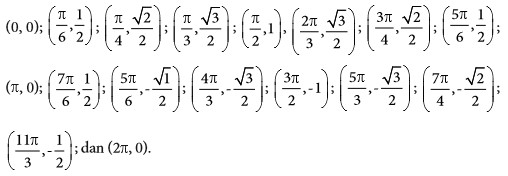
\includegraphics[scale=0.75]{fungsi_trigonometri_1}

Selanjutnya pada koordinat kartesius, kita menempatkan pasangan titiktitik untuk menemukan suatu kurva  yang melalui semua pasangan titik-titik tersebut. Selengkapnya disajikan pada Gambar berikut ini.\\

\begin{figure}[!ht]
\begin{center}
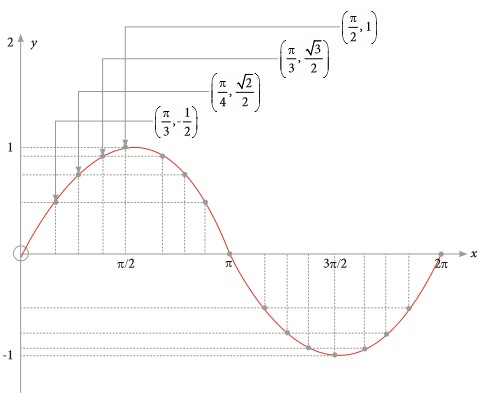
\includegraphics[scale=0.75]{grafik_fungsi_trigonometri_1}
\caption{Grafik fungsi $y = \sin x$, untuk $0 \leq x\leq 2\pi$}
\end{center}
\end{figure}

Dari grafik di atas,  kita dapat merangkum beberapa data dan informasi seperti berikut.
\begin{itemize}
\item Untuk semua ukuran sudut $x$,  nilai maksimum fungsi $y = \sin x$ adalah 1, dan nilai minimumnya adalah -1.
\item Kurva fungsi $y = \sin x$, berupa gelombang.
\item Untuk 1 periode (1 putaran penuh) kurva fungsi $y = \sin x$, memiliki 1 gunung dan 1 lembah.
\item Nilai fungsi sinus berulang saat berada pada lembah atau gunung yang sama.
\item Untuk semua ukuran sudut $x$, daerah hasil fungsi $y = \sin x$, adalah $1 \leq y \leq 1$. Dengan konsep grafik fungsi $y = \sin x$, dapat dibentuk kombinasi fungsi sinus.
\end{itemize}

Misalnya $y = 2.\sin x$, $y = \sin 2x$, dan $y = \sin (x+\pi/2)$ . Selengkapnya dikaji pada contoh berikut.

\begin{example}
Gambarkan grafik fungsi $y = \sin 2x$ dan $y = \sin (x+\pi/2)$, untuk $0 \leq x\leq 2\pi$. Kemudian tuliskanlah perbedaan kedua grafik tersebut.\\

\textbf{Alternatif Penyelesaian}\\
Dengan menggunakan nilai-nilai perbandingan trigonometri yang disajikan pada Tabel 4.3, maka pasangan titik-titik untuk fungsi $y = \sin 2x$, untuk $0 \leq x\leq 2\pi$ adalah:\\
Untuk $x = 0$, maka nilai fungsi adalah $y = \sin 2.(0) = \sin 0 = 0 \Rightarrow (0, 0)$\\
Untuk $x = (\pi/6)$, maka nilai fungsi adalah $y = \sin 2. (\pi/6) = \sin \pi/3 = \sqrt{3}/2 \Rightarrow(\pi/6,\sqrt{3}/2)$\\
Untuk $x = \pi/4$, maka nilai fungsi adalah $y = \sin 2. (\pi/4) = \sin \pi/2 = 1 \Rightarrow(\pi/4,1)$.\\
Demikian seterusnya hingga\\
untuk $x = 2\pi$, maka niali fungsi adalah $y = \sin 2.(2\pi) = \sin 4\pi = \sin 0 = 0 \Rightarrow (2\pi, 0)$\\
Selengkapnya pasangan titik-titik untuk fungsi $y = \sin 2x$, $0 \leq x\leq 2\pi$, yaitu

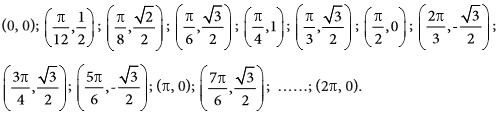
\includegraphics[scale=0.75]{fungsi_trigonometri_2}

Dengan  pasangan titik-titik tersebut, maka grafik fungsi $y = \sin 2x$, $0 \leq x\leq 2\pi$ disajikan pada Gambar.\\

\begin{figure}[!ht]
\begin{center}
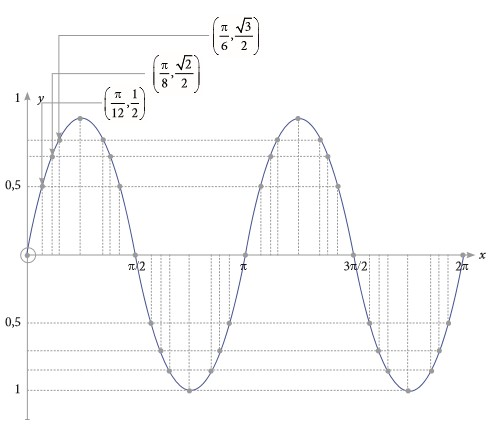
\includegraphics[scale=0.75]{grafik_fungsi_trigonometri_2} 
\caption{Grafik fungsi $y = \sin 2x$, untuk $0 \leq x\leq 2\pi$}
\end{center}
\end{figure}

Berbeda dengan fungsi $y = \sin 2x$, setiap besar sudut dikalikan dua, tetapi untuk fungsi $y = \sin(x+\pi/2)$, setiap besar sudut ditambah $\pi/2$ atau $90^o$.\\
Sekarang kita akan menggambarkan fungsi $y = \sin(x+\pi/2)$, untuk $0 \leq x\leq 2\pi$.\\
Coba kita perhatikan kembali, bahwa $\sin(x+\pi/2) = \cos x$. Artinya, sekarang kita akan menggambarkan fungsi $y = \cos x$, untuk $0 \leq x\leq 2\pi$. Dengan menggunakan nilai-nilai cosinus yang diberikan pada Tabel kita dapat merangkumkan pasangan titik-titik  yang memenuhi fungsi $y = \cos x$, untuk $0 \leq x\leq 2\pi$, sebagai berikut.

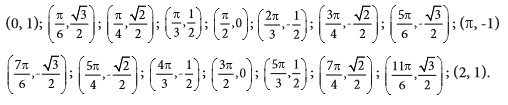
\includegraphics[scale=0.75]{fungsi_trigonometri_3}

Dengan demikian, grafik fungsi $y = \cos x$, untuk $0 \leq x\leq 2\pi$, disajikan pada Gambar berikut.\\

\begin{figure}[!ht]
\begin{center}
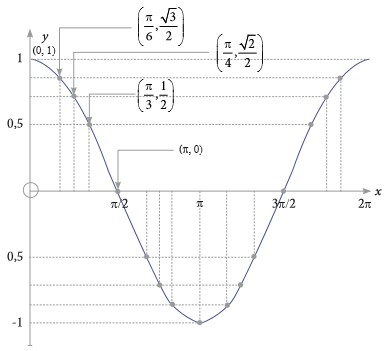
\includegraphics[scale=0.75]{grafik_fungsi_trigonometri_3} 
\caption{Grafik fungsi $y = \cos x$, untuk $0 \leq x\leq 2\pi$}
\end{center}
\end{figure}

Dari kajian grafik, grafik fungsi $y = \sin 2x$ sangat berbeda dengan grafik fungsi $y = \sin (x+\pi/2)  = \cos x$, meskipun untuk domain yang sama. Grafik $y = \sin 2x$, memiliki 2 gunung dan 2 lembah, sedangkan grafik fungsi $y = \sin (x+\pi/2)= \cos x$, hanya memiliki 1 lembah dan dua bagian setengah gunung. Nilai maksimum dan minimum fungsi $y = \sin 2x$ sama $y = \sin (x+\pi/2) = \cos x$ untuk domain yang sama. Selain itu, secara periodik, nilai fungsi $y = \sin 2x$ dan $y = \sin (x+\pi/2) = \cos x$, berulang, terkadang menaik dan terkadang menurun.
\end{example}
\begin{exercise}
Dengan pengetahuan dan keterampilan kamu akan tiga grafik di atas dan konsep yang sudah kamu miliki pada kajian fungsi, sekarang gambarkan dan gabungkan grafik $y = \sin x$ dan $y = \cos x$, untuk domain $0 \leq x\leq 2\pi$.\\
Rangkumkan hasil analisis yang kamu temukan atas grafik tersebut.
\end{exercise}
\item \textbf{Grafik Fungsi $y = tan x$, dan $y = \cos x$ untuk $0 \leq x\leq 2\pi$}\\
Kajian kita selanjutnya adalah untuk  menggambarkan grafik fungsi $y = \tan x$, untuk $0 \leq x\leq 2\pi$. Mari kita kaji grafik fungsi $y = \tan x$, melalui masalah berikut\\
\begin{problem}
Untuk domain $0 \leq x\leq 2\pi$, gambarkan grafik fungsi $y = \tan x$.\\
\end{problem}
\textbf{Alternatif Penyelesaian}\\
Dengan nilai-nilai tangen yang telah kita temukan pada Tabel 4.3 dan dengan pengetahuan serta keterampilan yang telah kamu pelajari tentang menggambarkan grafik suatu fungsi, kita dengan mudah memahami pasangan titik-titik berikut.\\

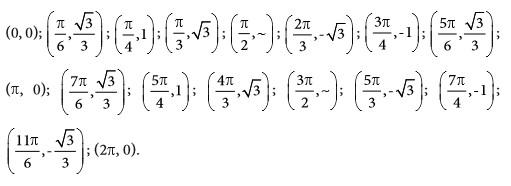
\includegraphics[scale=0.75]{fungsi_trigonometri_4}

Dengan demikian, grafik fungsi $y = \tan x$, untuk $0 \leq x\leq 2\pi$, seperti pada Gambar berikut ini.\\

\begin{figure}[!ht]
\begin{center}
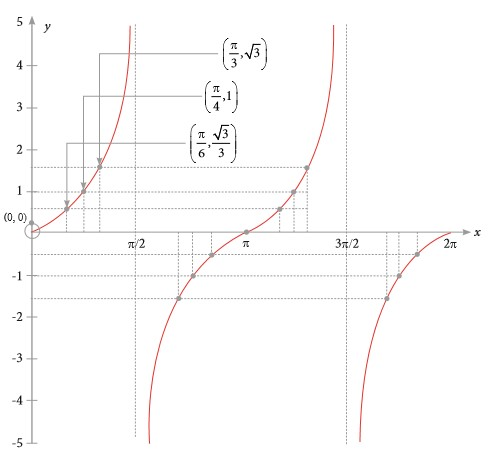
\includegraphics[scale=0.75]{grafik_fungsi_trigonometri_4} 
\caption{Grafik fungsi $y = \tan x$, untuk $0 \leq x\leq 2\pi$}
\end{center}
\end{figure}

Dari grafik di atas, jelas kita lihat bahwa jika $x$ semakin mendekati $\pi/2$ (dari kiri), nilai fungsi semakin besar, tetapi tidak dapat ditentukan nilai terbesarnya. Sebaliknya, jika $x$ atau mendekati $\pi/2$ (dari kanan), maka nilai fungsi semakin kecil, tetapi tidak dapat ditentukan nilai terkecilnya. Kondisi ini berulang pada saat $x$ mendekati $3\pi/2$. Artinya, fungsi $y = \tan x$, tidak memiliki nilai maksimum dan minimum.
\end{enumerate}
%------------------------------------------------
%----------------------------------------------------------------------------------------
%	BIBLIOGRAPHY
%----------------------------------------------------------------------------------------

\chapter*{Bibliography}
\addcontentsline{toc}{chapter}{\textcolor{ocre}{Bibliography}}
\section*{Books}
\addcontentsline{toc}{section}{Books}
\printbibliography[heading=bibempty,type=book]
\section*{Articles}
\addcontentsline{toc}{section}{Articles}
\printbibliography[heading=bibempty,type=article]

%----------------------------------------------------------------------------------------
%	INDEX
%----------------------------------------------------------------------------------------

\cleardoublepage
\phantomsection
\setlength{\columnsep}{0.75cm}
\addcontentsline{toc}{chapter}{\textcolor{ocre}{Index}}
\printindex

%----------------------------------------------------------------------------------------

\end{document}
